\documentclass[a4paper,11pt]{article}
\usepackage{graphicx}
\usepackage{enumerate}
\usepackage[usenames, dvipsnames]{color}
\usepackage[margin=1.25in]{geometry}
\usepackage{hyperref}

\usepackage{setspace}
\doublespacing

\begin{document}

\begin{flushright}

\vspace{1.1cm}

{\bf\Huge Hubble Space Telescope Spectra Database}

\rule{0.25\linewidth}{0.5pt}

\vspace{0.5cm}
%Put Authors
Justin Ely
\linebreak
%Put Author's affiliations
\footnotesize{605.411. Principles of Database Systems \\}
% Date here below
11 August, 2017
\end{flushright}

\noindent\rule{\linewidth}{1.0pt}

%------------------------------------------------------------------------------

\section{Introduction}
The Hubble Space Telescope (HST) is one of the most productive scientific instruments of all time, taking many observations each day and producing large quantities of data.  Unfortunately, the data storage for these archives grew organically over more than 25 years of operations.  This means the data is stored in a collection of ASCII files, binary files, and distributed databases with a large amount of redundancy and inneficiency. 

\subsection{Scope and Purpose of Document}
This document serves to describe the design and implementation of a database system to store and serve data for the Hubble Space Telescope.  Contained within are ER diagrams, operational rules, a sample implementation, and more to demonstrate applicability.  

\subsection{Project Objective}
This project aims to take a fresh look at storing this rich data archive with a focus on efficiency, integrity, and fast access access to help improve operations and use to the community.  Though this simple example, by restriction of scope, only applies to a fraction of the available data, the new approach can be expanded and applied to the entire archive.

%------------------------------------------------------------------------------
\section{System Requirements}
The requirements for deploying and running this database project are driven by the needs of the RDBMS employed.  For this project, PostgreSQL (postgres) was the RDBMS chosen.  A full listing of the most up-to-date technical requirements necessary should be checked at
\href{https://www.postgresql.org/}{https://www.postgresql.org/}, but an overview is provided here. 

\subsection{Hardware Requirements}
PostgreSQL supports many architectures including x86, ARM, PowerPC, and SPARC.  For development and testing of this project, an x86 Intel Core i7-4790K was employed.  

The database, as implemented at the time of this document, had a total size of 313728 bytes, or just over 300KB.  This is the very floor of free memory required to deploy the given database, but this represents just a small sample of the available data. A full production database would likely be many GB if the entire history of the telescope was to be injested.  The system used during development and test had 24GB of RAM and a 120GB SSD.  

\subsection{Software Requirements}
The postgres DBMS is well established and well supported.  It will run on Linux, OSX, and Windows, as well as many other UNIX varieties. Installing PostgreSQL requires GNU make and an ISO/ANSI C compiler.  The versions used for development were GNU Make 4.1 and GCC 5.4.0.  These were on an Ubuntu 16.04 64-bit system.

\subsection{Functional Requirements}
This application in general supports the storage and retrieval of HST spectral datasets and associated metadata.  This includes adding and tracking proposals, investigators, and targets with each new proposal cycle.  It also supports adding observations, their sub-exposures, and associated metadata as they are taken each day.  Finally, it supports statistical investigations and aggregations on the ingested data. 

\subsection{Database Requirements}
Postgres is an ORDBMS that has been in use for more than 20 years, and has wide community support.  It status as a reliable free and open-source tool was why it was chosen for this project.  Postgres v9.5.7 was used as the RDBMS for this project during development, but this is not known to be a hard dependency and the functionality is likely backwards and forwards compatible with many other versions.

%------------------------------------------------------------------------------
\section{Database Design Description}
\subsection{Design Rationale}
The design for the following ER model comes largely from a top-down approach; taking the existing largely flat archive of data and breaking it into smaller logical units to reduce duplication and increase performance.

The intent of this database is to present the information in as usefull a manner as possible; one that can be extended into many other uses.  To this end, as many entities as possible are non-identifying.  This lets each one stand a little better on it's own, and allow useful information retrieval without understanding another table.  Fortunately, this is possible for nearly all tables, with the notable exception of the detector entity, which needs its parent entity for unique identification.  Most entities also contained a unique attribute without needing to add a unique id using the DBMS.  The exceptions to this were the investigator, target, and description entities.

The entity with the most keys is the exposure, which maps most closely to the original source of data.  Many of the other entities are chunks of data that repeat for many exposure occurances, which is also why it has the most links to or from other entities.  

\subsection{E/R Model}
\subsubsection{Entities}
Investigator is an entity that represents a person with an accepted scientific proposal to use the telescope.  This entity gives each investigator a unique integer ID, and tracks their firstname, middlename, and lastname.

Proposal stores an accepted proposal for the telescope.  Each proposal has an unique integer ID (that has been assigned by another system), as well as the title.  A foreign key that references an investigator ID tracks which proposals were submitted by which Investigator.  An investigator may have many proposals, but a proposal may have only one investigator, so the proposal is a child entity of investigator.

Target is an entity which holds each unique astronomical target that has been observed.  Each has a unique ID, as well as its common name and position in right ascension and declination (ra and dec).  It is important to not use name or position by themselves as the unique identifier, as objects can move (i.e. jupiter) and will need multiple positions, and a particular line of sight (ra and dec) may contain many different objects.  Therefore, name or position alone cannot uniquely determine the target.   

Description holds individual human-given descriptions that can pertain to various astronomical observations.  Each entry has an ID and a description.  Descriptions can be any string description of an observed target or objects in the field.  Examples include, but are not limited to, planet, star, galaxy, nebule, bright, dim, etc.

The instrument entity holds entries for the scientific instruments that can be used in an observation.  This entity uses the instrument's name as a unique primary key, and holds pertinent metadata about the instrument such as sensitivity, manufacturer, installation date, and status.  

The instrument\_count entity holds a running total of the cumulative exposure time that has been observed for a given instrument.  This table is populated by a trigger that will be discussed in a later section.

The child entity of instrument is the detector entity.  Each scientific instrument can have multiple detectors.  This entity contains a compound primary key made of the detector name and the foreign key instrument ID.  The name of the detectors is not unique, but the instrument name + detector name is a unique combination.  The entity also contains detector-level metadata like the number of pixels and detector type.  

An exposure entity represents a unique activation of a detector on the telescope.  This entity represents a particular atomic "measurement" and the settings used.  Each exposure implementation was a unique ID, the date and time of the observation, as well has the configurations of MJD, exptime, observation mode, central wavelength used, and optical element in the beampath.  It also includes 3 foreign keys that link to the IDs for the instrument, detector and parent observation.

An Observation entity is a parent to the exposure entitiy. This entity is needed to group together many individual exposures and link them to proposals.  This grouping is needed as the observations listed in the proposal may in practice be broken up into multiple sub measurements (exposures) due to orbital constraints on continuous time segments.  

The file entity links each exposure to the physical file on disk that contains measurements and metadata. The primary key is the filename, which must be unique to avoid confusion, and a foreign key links it back to the exposure it informs.

Reference\_file entity tracks various permutable calibration switches that con control how the exposure data is reduced into it's final form.  Each reference file can apply to many individual exposures, or none, and each exposure will need many reference files.  

\subsubsection{Relationships}
Observes is a relationship that links targets to proposals.  This relationship is necessary because a proposal may have multiple targets, and a target may be observed in multiple proposals.  

Describes is a relationship that maps targets to descriptions with their respective IDs.  This relationship is necessary to resolve the many-to-many relationship that applies between these two entities.  

Applies\_to relates reference files and exposures.  Many reference files will apply to multiple exposures, and exposures will need to link to any number of reference files.  

\subsubsection{E/R Diagram}

\begin{figure}[h!]
\caption{ERD in IE notation for the HST spectra database.}
\centering
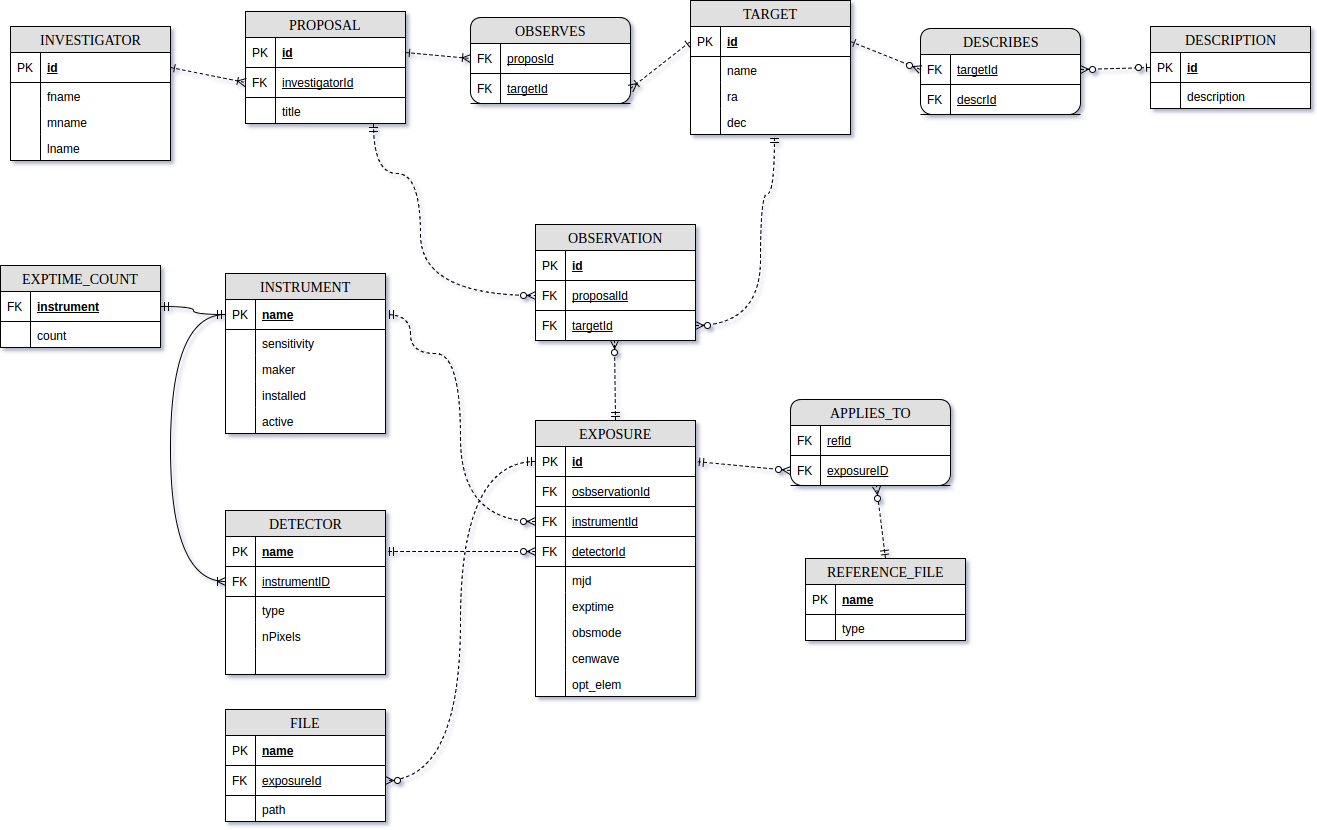
\includegraphics[width=.9\textwidth]{hst_spectra_erd.png}
\end{figure}

\subsection{Relational Model}
\subsubsection{Data Dictionary}
\hrulefill
APPLIES\_TO entity definition:
\begin{verbatim}
 Column |         Type          | Modifiers 
--------+-----------------------+-----------
 obs    | character(9)          | 
 ref    | character varying(30) | 
Foreign-key constraints:
    "applies_to_obs_fkey" FOREIGN KEY (obs) REFERENCES exposure(rootname)
    "applies_to_ref_fkey" FOREIGN KEY (ref) REFERENCES reference_file(name)

\end{verbatim}

\hrulefill

DESCRIPTION entity definition:
\begin{verbatim}
   Column    |         Type          |                        Modifiers                         
-------------+-----------------------+--------------------------------------
 id          | integer               | not null default 
                                       nextval('description_id_seq'::regclass)
 description | character varying(80) | 
Indexes:
    "description_pkey" PRIMARY KEY, btree (id)
Referenced by:
    TABLE "targ_map" CONSTRAINT "targ_map_descripid_fkey" 
    FOREIGN KEY (descripid) REFERENCES description(id)

\end{verbatim}

\hrulefill

DETECTOR entity definition:
\begin{verbatim}
 Column  |         Type          | Modifiers 
---------+-----------------------+-----------
 name    | character(4)          | not null
 inst    | character(4)          | not null
 npixels | integer               | 
 type    | character varying(20) | 
Indexes:
    "detector_pkey" PRIMARY KEY, btree (name, inst)
Check constraints:
    "detector_type_check" CHECK (type::text = 'mama'::text 
                              OR type::text = 'ccd'::text 
                              OR type::text = 'xdl'::text 
                              OR type::text = 'digicon'::text 
                              OR type::text = 'cathode'::text)
Foreign-key constraints:
    "detector_inst_fkey" FOREIGN KEY (inst) REFERENCES instrument(name)
Referenced by:
    TABLE "exposure" CONSTRAINT "exposure_detector_fkey" 
    FOREIGN KEY (detector, instrument) REFERENCES detector(name, inst)

\end{verbatim}

\hrulefill

EXPOSURE entity definition:
\begin{verbatim}
   Column   |         Type          | Modifiers 
------------+-----------------------+-----------
 rootname   | character(9)          | not null
 obsname    | character(9)          | 
 instrument | character(4)          | not null
 detector   | character(4)          | not null
 mjd        | double precision      | 
 exptime    | double precision      | 
 obsmode    | character varying(80) | 
 cenwave    | integer               | 
 opt_elem   | character(6)          | 
Indexes:
    "exposure_pkey" PRIMARY KEY, btree (rootname)
Check constraints:
    "exposure_cenwave_check" CHECK (cenwave > 0)
    "exposure_exptime_check" CHECK (exptime > 0::double precision)
    "exposure_mjd_check" CHECK (mjd > 0::double precision)
    "exposure_obsmode_check" CHECK (obsmode::text = 'ACCUM'::text 
                                 OR obsmode::text = 'TIME-TAG'::text)
Foreign-key constraints:
    "exposure_detector_fkey" FOREIGN KEY (detector, instrument) 
        REFERENCES detector(name, inst)
    "exposure_obsname_fkey" FOREIGN KEY (obsname) 
        REFERENCES observation(rootname)
Referenced by:
    TABLE "applies_to" CONSTRAINT "applies_to_obs_fkey" 
        FOREIGN KEY (obs) REFERENCES exposure(rootname)
    TABLE "file" CONSTRAINT "file_exposure_fkey" 
        FOREIGN KEY (exposure) REFERENCES exposure(rootname)
Triggers:
    add_exptime BEFORE INSERT ON exposure 
        FOR EACH ROW EXECUTE PROCEDURE log_exptime()

\end{verbatim}

\hrulefill

EXPTIME\_COUNT entity definition:
\begin{verbatim}
   Column   |       Type       | Modifiers 
------------+------------------+-----------
 instrument | character(4)     | 
 count      | double precision | 
Check constraints:
    "exptime_count_count_check" CHECK (count >= 0::double precision)
Foreign-key constraints:
    "exptime_count_instrument_fkey" FOREIGN KEY (instrument) REFERENCES instrument(name)
\end{verbatim}

\hrulefill

FILE entity definition:
\begin{verbatim}
  Column  |         Type          | Modifiers 
----------+-----------------------+-----------
 name     | character varying(30) | not null
 exposure | character(9)          | 
 fpath    | character varying(50) | 
Indexes:
    "file_pkey" PRIMARY KEY, btree (name)
Foreign-key constraints:
    "file_exposure_fkey" FOREIGN KEY (exposure) REFERENCES exposure(rootname)
\end{verbatim}

\hrulefill

INSTRUMENT entity definition:
\begin{verbatim}
  Column   |         Type          | Modifiers 
-----------+-----------------------+-----------
 name      | character(4)          | not null
 maker     | character varying(40) | 
 installed | double precision      | 
 active    | boolean               | 
Indexes:
    "instrument_pkey" PRIMARY KEY, btree (name)
Check constraints:
    "instrument_installed_check" CHECK (installed > 0::double precision)
Referenced by:
    TABLE "detector" CONSTRAINT "detector_inst_fkey" FOREIGN KEY (inst) REFERENCES instrument(name)
    TABLE "exptime_count" CONSTRAINT "exptime_count_instrument_fkey" FOREIGN KEY (instrument) REFERENCES instrument(name)
\end{verbatim}

\hrulefill

INVESTIGATOR entity definition:
\begin{verbatim}
 Column |         Type          |                         Modifiers                         
--------+-----------------------+-----------------------------------------------------------
 id     | integer               | not null default nextval('investigator_id_seq'::regclass)
 fname  | character varying(30) | 
 mname  | character varying(30) | 
 lname  | character varying(30) | 
Indexes:
    "investigator_pkey" PRIMARY KEY, btree (id)
Referenced by:
    TABLE "proposal" CONSTRAINT "proposal_pi_fkey" FOREIGN KEY (pi) REFERENCES investigator(id)
\end{verbatim}

\hrulefill

OBSERVATION entity definition:
\begin{verbatim}
      Table "public.observation"
   Column   |     Type     | Modifiers 
------------+--------------+-----------
 rootname   | character(9) | not null
 proposalid | integer      | 
Indexes:
    "observation_pkey" PRIMARY KEY, btree (rootname)
Foreign-key constraints:
    "observation_proposalid_fkey" FOREIGN KEY (proposalid) 
        REFERENCES proposal(proposid)
Referenced by:
    TABLE "exposure" CONSTRAINT "exposure_obsname_fkey" 
        FOREIGN KEY (obsname) 
        REFERENCES observation(rootname)
\end{verbatim}

\hrulefill


PROPOSAL entity definition:
\begin{verbatim}
  Column  |         Type          | Modifiers 
----------+-----------------------+-----------
 proposid | integer               | not null
 pi       | integer               | not null
 title    | character varying(80) | 
Indexes:
    "proposal_pkey" PRIMARY KEY, btree (proposid)
Check constraints:
    "proposal_proposid_check" CHECK (proposid > 0)
Foreign-key constraints:
    "proposal_pi_fkey" FOREIGN KEY (pi) REFERENCES investigator(id)
Referenced by:
    TABLE "observation" CONSTRAINT "observation_proposalid_fkey" 
    FOREIGN KEY (proposalid) 
    REFERENCES proposal(proposid)
\end{verbatim}

\hrulefill


REFERENCE\_FILE entity definition:
\begin{verbatim}
 Column |         Type          | Modifiers 
--------+-----------------------+-----------
 name   | character varying(30) | not null
 type   | character varying(30) | 
Indexes:
    "reference_file_pkey" PRIMARY KEY, btree (name)
Referenced by:
    TABLE "applies_to" CONSTRAINT "applies_to_ref_fkey" 
      FOREIGN KEY (ref) 
      REFERENCES reference_file(name)

\end{verbatim}

\hrulefill

DESCRIBES entity definition:
\begin{verbatim}
  Column   |  Type   | Modifiers 
-----------+---------+-----------
 targetid  | integer | 
 descripid | integer | 
Foreign-key constraints:
    "targ_map_descripid_fkey" FOREIGN KEY (descripid) 
        REFERENCES description(id)
    "targ_map_targetid_fkey" FOREIGN KEY (targetid) 
        REFERENCES target(id)
\end{verbatim}

\hrulefill

TARGET entity definition:
\begin{verbatim}
 Column |         Type          |                      Modifiers                      
--------+-----------------------+-----------------------------------------------------
 id     | integer               | not null default 
                                  nextval('target_id_seq'::regclass)
 name   | character varying(30) | 
 ra     | double precision      | 
 dec    | double precision      | 
Indexes:
    "target_pkey" PRIMARY KEY, btree (id)
Referenced by:
    TABLE "targ_map" CONSTRAINT "targ_map_targetid_fkey"
       FOREIGN KEY (targetid) REFERENCES target(id)
\end{verbatim}

\hrulefill

\subsubsection{Integrity Rules}
Integrity rules for this database are enforced with on the tables themselves, with primary and foreign keys, unique/not null constraints, and specific data constraints. Much of the concern with this database is keeping referential integrity between all the linked entities.  A strong set of primary and foreign keys keeps this together by ensuring that the linkages will exist with each insertion.  

Additionally, specific column constraints were used throughout for individual data integrity.  Typical examples are constraining columns to a few known values, like in the detector.type attribute.  Other constraints simply make sure the data is within known ranges, like enforcing non-negative values for exposure.exptime.  Since a negtive exposure time is physically impossible, and this attribute is often used in calculations, catching an improper value early is very valuable. 

\subsubsection{Operational Rules}
Operational rules are rather permitting for this application, as it's designed to be flexible and permit the aggregation of disparate, but linked, data.  As such, operations are permitted so long as the do not violate the data integrity rules built into the table.  I.e. a proposal may not be added into the system either creating a new or linking to an existing investigator, due to the foreign key constraint. Similarly, an exposure cannot be inserted without a linked observation which can't be inserted without an existing proposal.  The hierarchy of keys and constraints enforce the operational rules, but anything else is permitted. 

\subsubsection{Operations}
A common operation that will be performed on this database is the insertion of the proposals from a recent round of approvals.  This operation involves inserting any new investigators, inserting new proposals, then reading the target table and linking or inserting as needed.   

\subsection{Security}
For this database, security is a minor concern.  All data used is public-domain, so access control is not required.  In addition, the database is an abstract layer on top of existing data products designed to be more efficient and easy-to-use, but it is not the sole point of truth.  Therefore, the database can easily be re-created from the source should any data be lost.  In addition, the database is not currently hosted, so preventing malicious access is a minor concern.

\subsection{Database Backup and Recovery}
Backup will be accomplished through the PG\_DUMP task.  This is a utility included with PostgreSQL that dumps the entire database contains into plaintext suitable to re-create the entire state of the database.  This backup is performant at these small scales, but has not been tested with a larger database.  However, given the infrequent additions to the database in a production environment, a low performance dump will not hamper operations.  

\subsection{Using Database Design or CASE Tool}
Entities and the ERD were created with \href{https://draw.io}{draw.io}, and database administration was done through the command-line tools provided by PostgreSQL.  While many more fully-featured tools may have made these tasks easier, I prefer to learn directly with the tools themselves.  Activities like installing the DBMS, creating users, adding tables, inserting data, and all other activities were done by hand. 

\subsection{Other Possible E/R Relationships}
An additional E/R relationship that could be useful to implement would be to add an Institution entity and a works\_for relationship to the existing investigor entity.  This would allow additional reporting like which institutions around the world were more or less successful at proposing in a given year. 

I also considered a completely different ERD where the tables much more closely resembled the existing file structures as produced by the mission.  This then produced an ERD centered almost entirely on observations, and suffered from a great deal of data redundancy and difficult queries. 

%------------------------------------------------------------------------------
\section{Implementation Description}
\subsection{Data Dictionary}
\begin{verbatim}
spec=# \dt+
                          List of relations
 Schema |      Name      | Type  | Owner  |    Size    | Description 
--------+----------------+-------+--------+------------+-------------
 public | applies_to     | table | justin | 120 kB     | 
 public | description    | table | justin | 8192 bytes | 
 public | detector       | table | justin | 8192 bytes | 
 public | exposure       | table | justin | 8192 bytes | 
 public | exptime_count  | table | justin | 40 kB      | 
 public | file           | table | justin | 40 kB      | 
 public | instrument     | table | justin | 8192 bytes | 
 public | investigator   | table | justin | 8192 bytes | 
 public | observation    | table | justin | 8192 bytes | 
 public | proposal       | table | justin | 8192 bytes | 
 public | reference_file | table | justin | 40 kB      | 
 public | targ_map       | table | justin | 8192 bytes | 
 public | target         | table | justin | 8192 bytes | 

\end{verbatim}

\subsection{Advanced Features}
This database contains stored functions and triggers to perform automatic data aggregation as inserts occur.  The stored procedure updates a row in a table that stores the total accumulated exposure time for a given instrument.  The trigger, causes the procedure to run each time a new exposure is added to the exposure table.  This way, when new data is taken, the exposure time is automatically added to a running total in another entity, and the aggregate stats are always up-to-date.  The features are defined as follows.

\begin{verbatim}
-- stored procedure
CREATE FUNCTION log_exptime() RETURNS trigger AS $log_exptime$
BEGIN
  UPDATE exptime_count SET count = (count + NEW.exptime)
    WHERE instrument = NEW.instrument;
  RETURN NEW;
END;
$log_exptime$ LANGUAGE plpgsql;
  
-- DB trigger
CREATE TRIGGER add_exptime
  BEFORE INSERT ON exposure FOR EACH ROW EXECUTE PROCEDURE log_exptime();
\end{verbatim}

\subsection{Queries}
\subsubsection{Describing a target}
This query would be very common, as astronomical names are not terribly descriptive as to what the source is.  Not only that, but a field of view can be very large, so multiple different objects may be visible.  Therefore, mapping an individal target through all available descriptions is useful to understand what is being looked at. 

\begin{verbatim}
spec=# SELECT description FROM target 
              JOIN targ_map ON target.id=targ_map.targetid 
              JOIN description ON descripid=description.id 
              WHERE name = 'NGC-7469';
			
 description 
-------------
 NLR
 BLR
 SEYFERT
 NUCLEUS
(4 rows)
\end{verbatim}

\subsubsection{Find applicable reference files for an exposure}
Each exposure has been calibrated from the raw data down to a useable form.  It is common to need to back-track and understand what was applied to the data, so mapping an exposure to all applicable reference material is useful to fully understand the data.

\begin{verbatim}
spec=# SELECT ref FROM exposure 
              JOIN applies_to ON rootname=obs 
              WHERE rootname='lc7001b3q';
			
         ref          
----------------------
 xab1551cl_flat.fits
 u1t1616ql_wcp.fits
 1811831fl_spwcs.fits
 14o2013ql_xwalk.fits
 14o2013rl_ywalk.fits
 0561933ll_tds.fits
 lc7001050_asn.fits
 0bn1606sl_disp.fits
 zas1615jl_spot.fits
 1811827rl_lamp.fits
 x6q17586l_1dx.fits
 wc318317l_pha.fits
 x1u1459il_brf.fits
 0561933jl_phot.fits
 yae1249sl_bpix.fits
 s7g1700gl_dead.fits
 zbn1927gl_gsag.fits
 x1u1459gl_geo.fits
\end{verbatim}

\subsubsection{Which investigator has the most observing time}
This query may be of use for general stats, and/or to help in investigating bias among proposal selection commitees.  

\begin{verbatim}
spec=# SELECT fname, mname, lname, SUM(exptime) FROM investigator 
              JOIN proposal on id=pi 
              JOIN observation ON proposid=observation.proposalid 
              JOIN exposure ON observation.rootname=obsname 
              GROUP BY fname, mname, lname 
              ORDER BY sum DESC;

   fname   | mname |  lname   |     sum      
-----------+-------+----------+--------------
 Jelle     |       | Kaastra  |        23615
 Nahum     |       | Arav     |        23085
 Francesco |       | Palla    | 13856.199951
 Reginald  | J.    | Dufour   |       2634.5
 Guy       |       | Worthey  |          165
 Charles   | R.    | Proffitt |          0.1
(6 rows)
\end{verbatim}

\subsubsection{Rank investigators by number of successful proposals}
Similar to the query above, this ranks all investigators instead by the number of succesffuly proposals.  This would be used as another metric as general stats or helping to understand bias/demographics/usage/etc.  

\begin{verbatim}
SELECT fname,mname, lname, COUNT(*) FROM investigator 
       JOIN proposal ON id=pi 
       GROUP BY fname, mname, lname 
       ORDER BY count DESC;

   fname   | mname |  lname   | count 
-----------+-------+----------+-------
 Nahum     |       | Arav     |     2
 Guy       |       | Worthey  |     1
 Jelle     |       | Kaastra  |     1
 Charles   | R.    | Proffitt |     1
 Francesco |       | Palla    |     1
 Reginald  | J.    | Dufour   |     1
(6 rows)

\end{verbatim}

\subsubsection{Find which instrument is most used}
This is a very common query to determine which instrument is most widely used by raw exposure time.  This information is important for understanding the needs of the community, as well as tracking the degredation of the instrument being used.

\begin{verbatim}
spec=# SELECT * FROM exptime_count ORDER BY count DESC LIMIT 1;

 instrument | count 
------------+-------
 COS        | 46700
(1 row)
\end{verbatim}


%------------------------------------------------------------------------------
\section{CRUD Matrix}
\begin{center}
 \begin{tabular}{||c c c c c c||} 
 \hline
 & applies\_to & description & detector & exposure & exptime\_count \\ [0.5ex] 
 \hline\hline
 F1 & & & & & \\ 
 \hline
 F2 & R &  & R & C & U \\  
 \hline
 F3 & & & & D & U \\  
 \hline
\end{tabular}
\end{center}

\begin{center}
 \begin{tabular}{||c c c c c c c||} 
 \hline
 & file & instrument & investigator & observation & proposal & reference\_file \\ [0.5ex] 
 \hline\hline
 F1 & & & R & & C & \\
 \hline
 F2 & C & R & & R & & RC \\
 \hline
 F3 & D & & & & & \\ 
 \hline
\end{tabular}
\end{center}

\subsection{List of Entity Types}
\begin{itemize}
	\item applies\_to
 	\item description
 	\item detector
 	\item exposure
 	\item exptime\_count
 	\item file
 	\item instrument
 	\item investigator
 	\item observation
 	\item proposal
 	\item reference\_file
 	\item targ\_map 
 	\item target 
\end{itemize}
\subsection{List of Functions}
\begin{itemize}
	\item F1: Insert a new proposal.
 	\item F2: Insert a new exposure.
 	\item F3: Delete an exposure.
\end{itemize}

%------------------------------------------------------------------------------
\section{Concluding Remarks}
This project was an interesting exploration into how to re-organize and optimize an existing collection of data into a new database format.  I learned much from this project in regards to actual SQL capabilities and DBMS peculiarities.

The capabilities of triggers and stored procedures was new for me, but the usefulness was immediately obvious.  Especially for a project like this, where many derived attributes can be calculated on the fly as things are inserted.  This can save outside users from having to learn too much syntax, if common calculations can be automatic.  This can also help performance in large DB by "pre-calculating" certain things that are more intensive.  Unfortunately, I didn't implement very many in this project, but that would be a key expansion to a follow-up on this topic.  

PostgreSQL is a powerful database, and I found no issues when using it for typical SQL like INSERT, UPDATE, SELECT, etc.  However, I find that I don't as much like the DBA tools built-in.  The syntax very much breaks from typical SQL, and if feels far more like switching languages than the corresponding tasks in tools like MySQL or Sqlite.  Though it's good to be exposed to other tools, in the future I will likely stick more to MySQL if possible, as I vastly prefer the DBA syntax.  

\pagebreak

\appendix
%------------------------------------------------------------------------------
\section{DDL, INSERT, SELECT Statements}
The DDL, INSERT, SELECT statements necessary to create the database are over 2000 lines long. This would make the report unnecessarily long, so they have been hosted in a public Github repository for viewing. They can be found at \href{https://github.com/justincely/hst\_db\_project}{https://github.com/justincely/hst\_db\_project}.



\end{document}
